\begin{frame}
  \frametitle{The \gls{PCC} magnitudes show the most sensitive \glspl{DNP}}
  \begin{columns}
    \column[t]{0.67\textwidth}
  \begin{figure}[!ht]
    \centering
    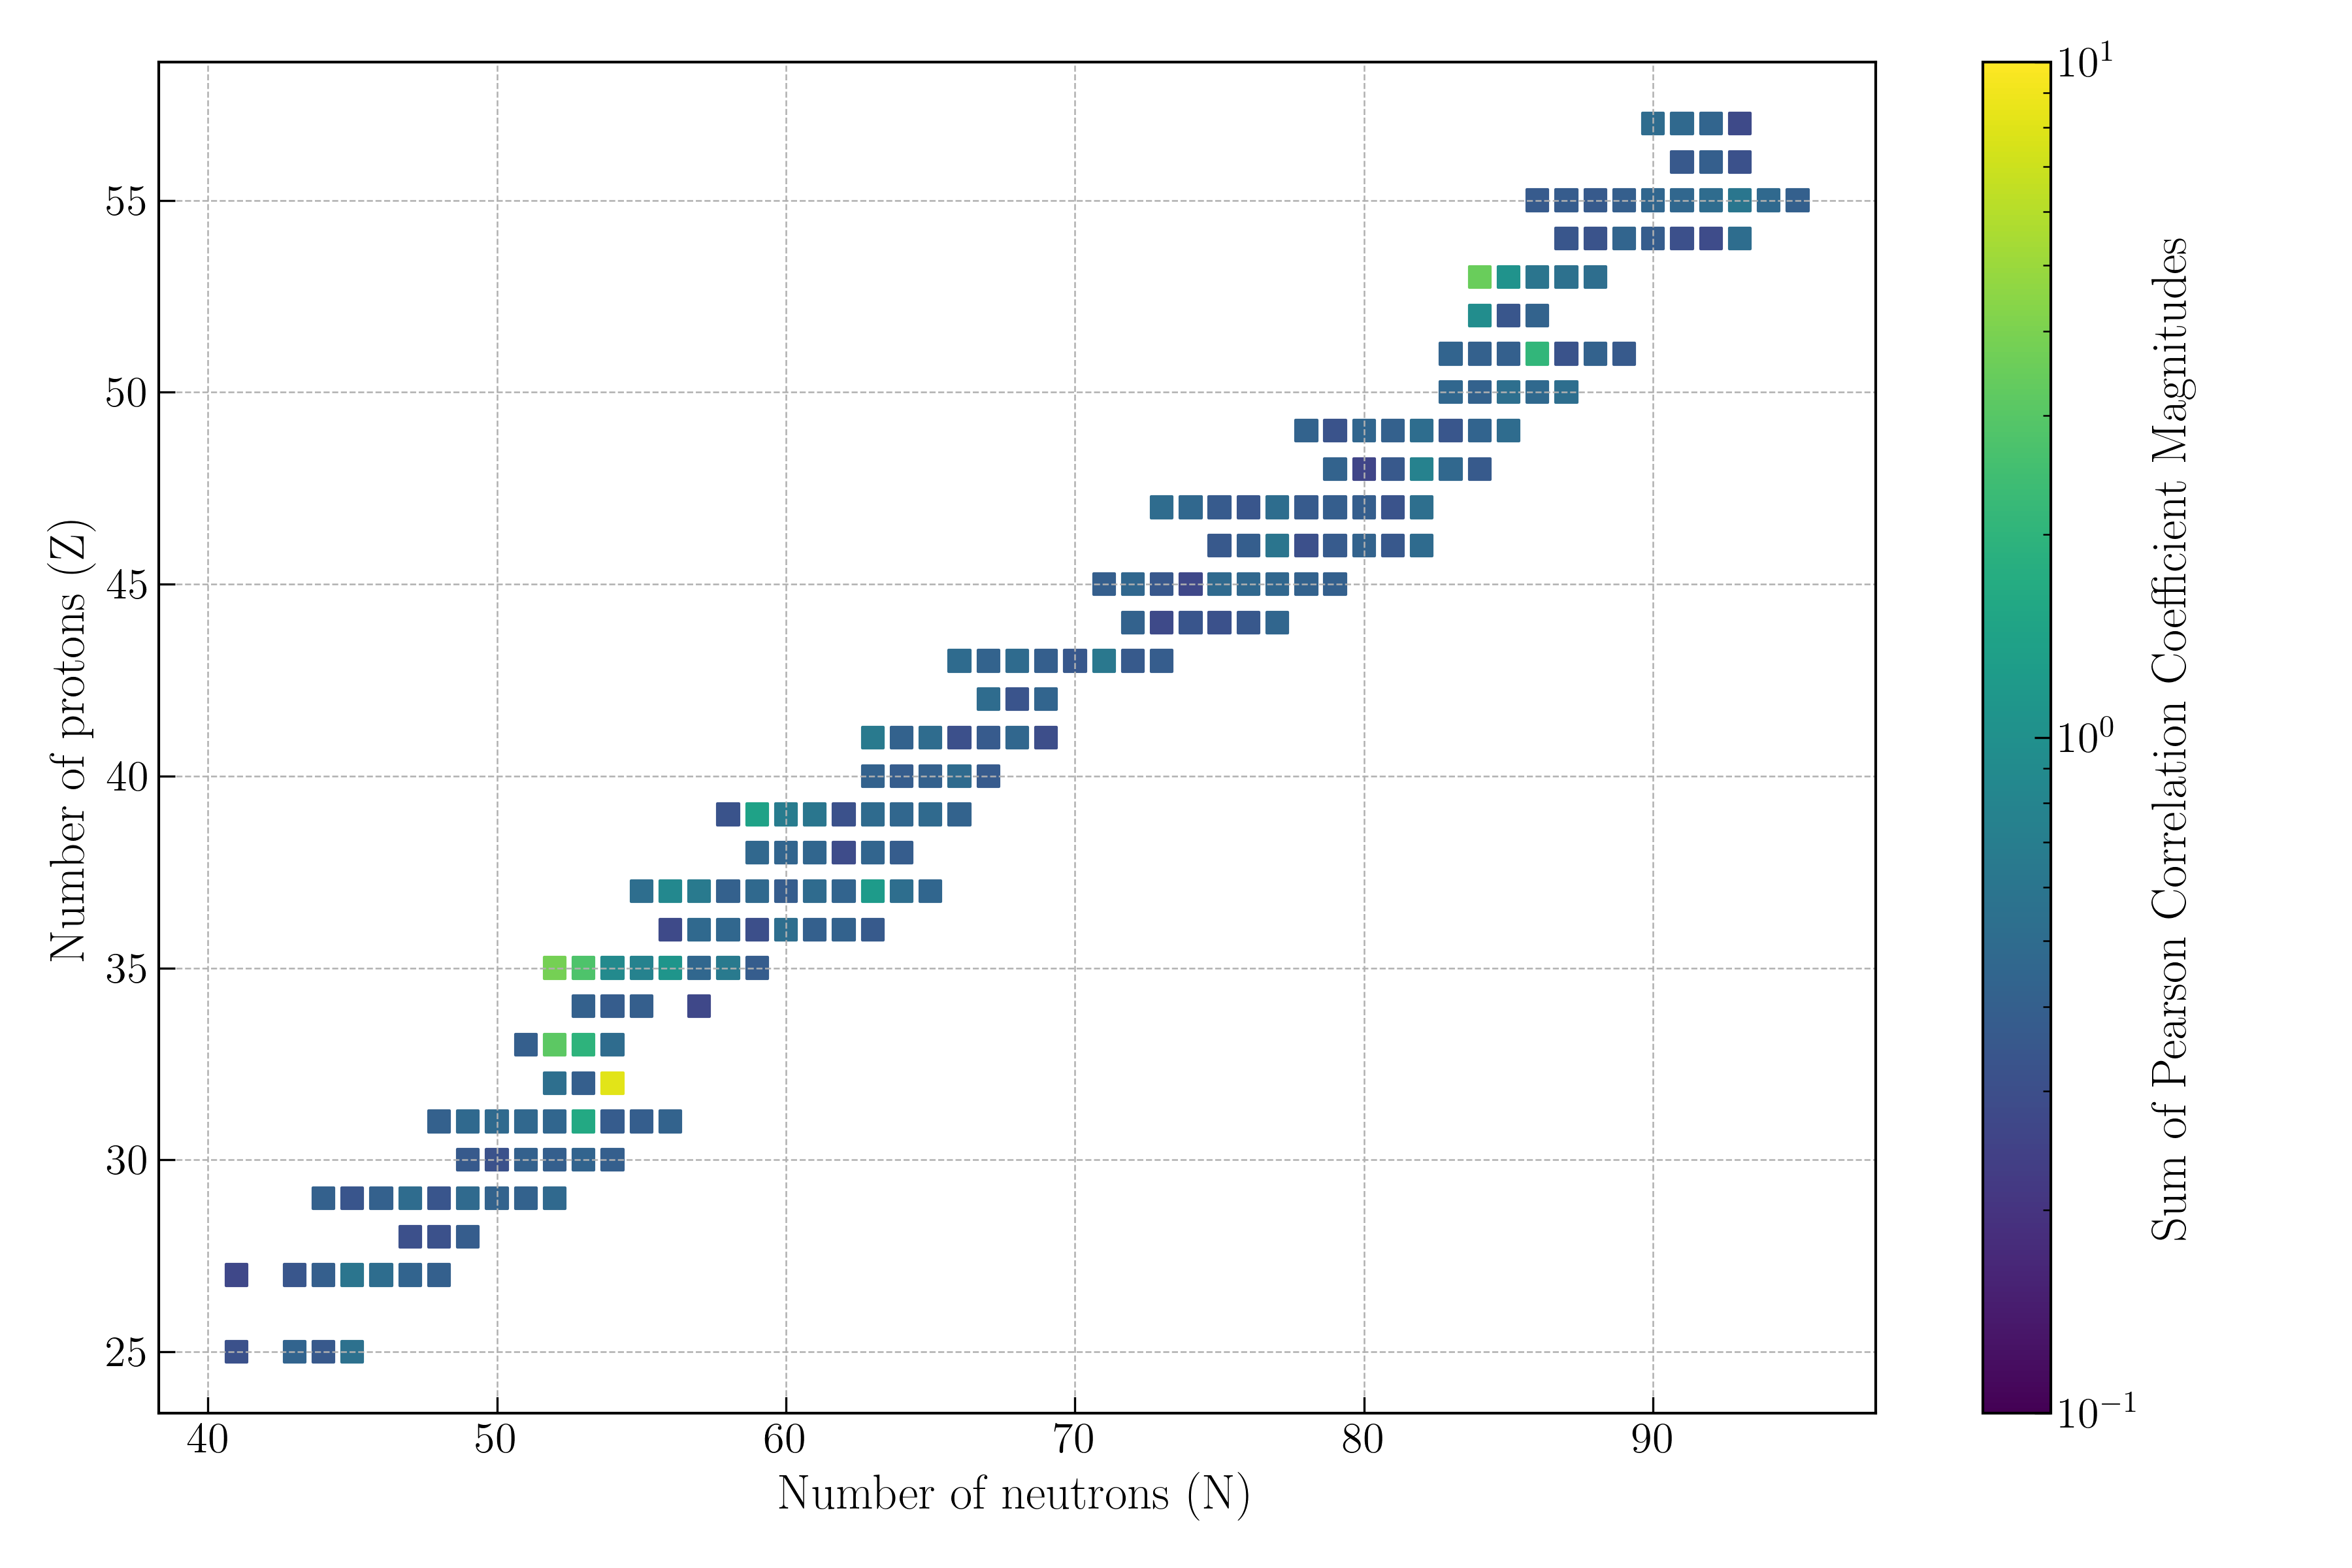
\includegraphics[width=0.95\linewidth]{../images/chart_PCC.png}
    \caption{The summed \gls{PCC} magnitudes after a thermal saturation irradiation of $^{235}$U using the 0D scaled model.}
    \label{fig:summedpccs}
    \end{figure}
    \column[t]{0.33\textwidth}
    \begin{table}[!ht]
    \centering
    \caption{The largest summed \gls{PCC} magnitudes after a thermal saturation irradiation of $^{235}$U using the 0D scaled model.}
\begin{tabular}{lr}
\hline
Nuclide &  $PCC_{i}$ \\
\hline
$^{86}$Ge & 8.06 \\
$^{87}$Br & 3.82 \\
$^{137}$I & 3.52 \\
$^{85}$As & 3.14 \\
$^{88}$Br & 2.77 \\
$^{137}$Sb & 2.08 \\
$^{86}$As & 1.97 \\
$^{84}$Ga & 1.62 \\
$^{98}$Y & 1.42 \\
$^{100}$Rb & 1.22 \\
\hline
\end{tabular}
\label{tab:pcc-summed}
\end{table}
  \end{columns}

\end{frame}

